% =============================================================================
%  Body-first layout draft -- "Rank Before You Merge"
%  Main paper only: one measured method figure, no appended supplement.
%  Double-blind review mode.
%
%  DISCIPLINE (do not violate when editing):
%   - Every NUMBER is copied verbatim from the markdown source. Do not change.
%   - Red-line wording (scoped claims, the locked cascade-gate quote, the GQA
%     single-full-statement, "robust default, not uniformly optimal") is
%     copied verbatim. Do not weaken.
%   - Double-blind: NO author / repository / institution / internal digest path
%     appears anywhere in this file. The "Source: *.md" provenance lines of the
%     markdown (work notes) are intentionally NOT typeset here.
%
%  FIGURE: fig1.pdf is the measured Qwen3-VL-8B merger-input/output L2
%  comparison on one real image (df7282e1, 25% kept). Later result figures are
%  intentionally deferred until their visual design is settled.
%
%  PAGE BUDGET (hard cap: <=8 pp body + <=2 pp refs). Compression points already
%   applied are marked  % [COMPRESSED ...] ; further optional levers are marked
%   % [COMPRESS-OPTIONAL ...] for the user to apply if the actual compile runs
%   long (see README_compile.txt, "if it overflows").
% =============================================================================

\documentclass[sigconf,review,anonymous]{acmart}

% --- packages actually used in this file -------------------------------------
\usepackage{booktabs}     % \toprule \midrule \bottomrule (acmart also loads it)
\usepackage{multirow}     % Table 1 / Table 3 model-column row spans
\usepackage{algorithm}    % Algorithm 1 float
\usepackage{algorithmic}  % Algorithm 1 pseudocode
\usepackage{pifont}       % \ding{51}=check, \ding{55}=cross (replaces emoji)
\usepackage{graphicx}     % \includegraphics (figures), \fbox placeholders
\usepackage{url}          % \path{} for any path-like strings

% --- review / submission front-matter hygiene --------------------------------
\setcopyright{none}
\settopmatter{printacmref=false, printccs=true, printfolios=true}

% --- CCS concepts (metadata only; regenerate via the ACM CCS tool if desired) -
\begin{CCSXML}
<ccs2012>
<concept>
<concept_id>10010147.10010257</concept_id>
<concept_desc>Computing methodologies~Machine learning</concept_desc>
<concept_significance>500</concept_significance>
</concept>
<concept>
<concept_id>10010147.10010375</concept_id>
<concept_desc>Computing methodologies~Computer vision</concept_desc>
<concept_significance>500</concept_significance>
</concept>
<concept>
<concept_id>10010147.10010172</concept_id>
<concept_desc>Computing methodologies~Natural language processing</concept_desc>
<concept_significance>300</concept_significance>
</concept>
</ccs2012>
\end{CCSXML}
\ccsdesc[500]{Computing methodologies~Machine learning}
\ccsdesc[500]{Computing methodologies~Computer vision}
\ccsdesc[300]{Computing methodologies~Natural language processing}

\keywords{visual token compression, vision-language models, training-free
  inference, multimodal foundation models, inference efficiency}

% =============================================================================
\begin{document}

\title[Rank Before You Merge]{Rank Before You Merge: A Stage Law for Training-Free Visual Token
  Compression in Merger-Equipped Vision-Language Models}

% Double-blind: the [anonymous] option anonymizes this automatically; the
% placeholder below is the de-anonymization stub.
\author{Anonymous Author(s)}
\renewcommand{\shortauthors}{Anonymous}
\affiliation{%
  \institution{Anonymous Affiliation}
  \country{}
}

% -----------------------------------------------------------------------------
\begin{abstract}
Merger-equipped vision-language models (VLMs) treat their native merger as
lossless; on text-dense workloads it is not. We isolate the \emph{stage} at
which token selection happens --- before or after that merger --- as an
experimental variable under iso-model / iso-token / iso-selector control, and
lead with the causal evidence. \textbf{(1) A selection-level causal
mechanism.} The learned merger reshuffles unit ranks almost from scratch
(Spearman $\rho = 0.14$--$0.36$) and, on documents, systematically demotes
text-stroke units; a ranking-swap control recovers pre-merger accuracy exactly,
and the two stages keep \emph{identical} unit sets (Jaccard $= 1.000$ on both
architectures tested): the kept-set identity --- not the selector identity,
not the forward path --- decides the outcome, so the entire pre$>$post gap is
the ranking the merger rewrites. \textbf{(2) A stage law as the mechanism's
generality.} Query-blind pre-merger selection systematically leads post-merger
selection on text-dense workloads --- $+11.0$ to $+38.4$~pp across two Qwen-VL
generations (full splits, paired McNemar $|z| \geq 14.6$) and $+37.4 /
+34.6$~pp with $+432$~pts on a third family, InternVL3-8B (a different merger
design: pixel-shuffle rather than Qwen's PatchMerger), under iso-selector /
iso-budget control; a fourth, fully independent lineage
(GLM-4.1V-9B-Thinking) replicates the text-dense pre$\gg$post effect in an
$n = 200$ gate (GQA arm inconclusive under the deterministic greedy
protocol). There is no text-dense crossover at the native-resolution
full splits (one shallow 600k-cap DocVQA configuration reverses; configuration
boundary in \S\ref{sec:discussion}), the gap widens monotonically under
compression, and object-centric GQA shows at most a small significant
post-stage edge (Qwen $+2.6$--$2.8$~pp) or a tie (InternVL3, $-0.4$~pp).
\textbf{(3) A closed design space and a regime map.} Four pre-registered
extensions --- QA-gate, hybrid mask, image router, two-stage cascade --- all
fail on the families/configurations tested (measured on Qwen3-VL, the cascade
under a locked gate): pre-merger selection behaves as a fixed point that no
downstream selector we tried improves. The method, Rank-Before-Merge (RBM), is
a query-blind, OCR-preserving robust default for text-dense workloads --- a
robust default, not uniformly optimal: the query-conditioned strong baseline
  FastV wins most reference-grounded cells (all three on Qwen3-VL and TextVQA
  on Qwen2.5-VL), while RBM uniquely retains dense OCR --- and 25\%-retention compression is
stage-neutral, raising throughput $+68\%$ (Qwen) / $1.8$--$2.5\times$ req/s
(InternVL3). Code will be released.
\end{abstract}

\maketitle

% FIG 1 -- enqueue immediately after the title so the two-column float lands
% reliably at the top of page 2.
\begin{figure*}[!t]
  \centering
  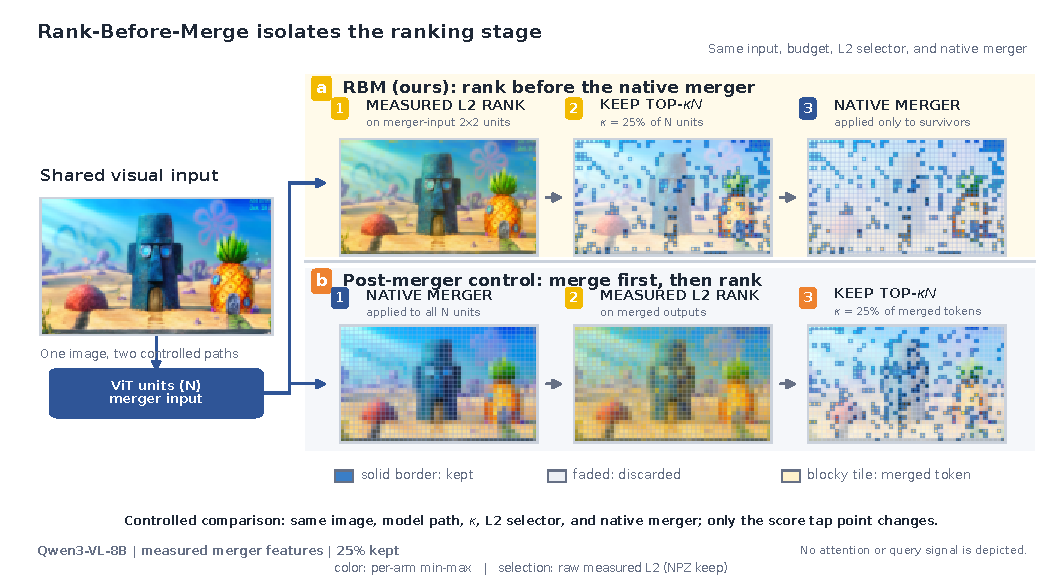
\includegraphics[width=\textwidth]{figs/fig1.pdf}
  \Description{A two-row comparison of visual-token selection before and after
    a VLM's native merger, using the same image, L2 selector, and token budget.}
  \caption{Rank-Before-Merge isolates the selection stage under
    iso-model, iso-token, and iso-selector control. The visualization uses
    measured Qwen3-VL-8B features from one real image ($N=1144$ merge units;
    25\% retained). Both rows use the same query-blind L2 selector and the
    unmodified native merger. RBM ranks merger-input units and merges only the
    survivors; the post control merges first and then ranks the resulting
    tokens. Solid cells are retained and faded cells are discarded. Equal
    output token counts but different masks expose merger-induced rank
    reordering; no attention or query signal is used.}
  \label{fig:fig1}
\end{figure*}

% =============================================================================
\section{Introduction}\label{sec:intro}
% =============================================================================

\textbf{Multimodal inference cost is a visual-token problem.} Vision-language
models (VLMs) have become a core class of multimodal foundation models, but an
image enters the language model as hundreds to tens of thousands of visual
tokens, and the quadratic attention cost and the key-value memory of these
tokens dominate multimodal inference. Visual-token compression --- pruning or
merging the least important tokens before or within the language model --- is
therefore a standard efficiency lever, with direct consequences for document
understanding, scene-text question answering, and OCR, the most token-hungry
multimodal workloads. In merger-equipped architectures --- the Qwen-VL family,
InternVL3, and others that merge $2\!\times\!2$ patch groups into one token ---
the compression debate has run almost entirely over \emph{which} tokens to keep
and \emph{how} to score them. The \emph{stage} at which selection happens,
before or after the native merger, has not been isolated as an experimental
variable, even though practitioners knew the merger matters: the Qwen2.5-VL
authors themselves note it already compresses, and merging is reported to
degrade OCR. Yet the working assumption behind this literature is that the
native merger is lossless --- select after it, and only the scorer matters.
Our first result overturns that assumption, and the evidence is causal, not
correlational (Figure~\ref{fig:fig1}).

\textbf{What we find first --- a selection-level causal mechanism.} The
pre-vs-post gap is not information destroyed in the forward pass; it is a
rewritten ranking, and we can say so causally. \textbf{M1:} the learned merger
reshuffles unit saliency almost from scratch --- pre- and post-merger unit
ranks agree only weakly (Spearman $\rho = 0.14$--$0.36$) --- most on documents,
least on object scenes. \textbf{M2:} on documents, the units the merger demotes
are precisely the high-edge text-stroke units, so post-merger selection is
systematically anti-text. \textbf{M3:} a ranking-swap control --- run the
post-merger forward path but select units with the pre-merger ranking ---
recovers pre-merger accuracy exactly (DocVQA 200/200 byte-identical answers;
TextVQA 198/200), and the two paths keep \emph{exactly the same} unit sets
(kept-set Jaccard $= 1.000$ in all four model$\times$benchmark cells on both
architectures). The verdict is \textbf{kept-set identity, not selector
identity}: the same L2 selector at both stages produces opposite outcomes
because the merger rewrites the ranking it acts on, and restoring the
pre-merger ranking alone --- same selector family, same forward path ---
restores the accuracy. Where tested byte-exactly (Qwen3-VL), the merged
representations of kept units carry no stage-dependent loss; selection order,
not the forward path, is the lever (\S\ref{sec:mechanism}).

\textbf{What falls out of it --- a stage law across families.} The mechanism's
benchmark-level consequence is a stage law: under strict iso-model / iso-token /
iso-selector control, applying the \emph{same} text-agnostic L2 scorer before
the merger versus after it --- iso-budget, so a pure stage variable ---
produces a large accuracy gap on text-dense benchmarks and at most a small,
reversed gap on object-centric GQA. On the official full splits, pre-merger
selection leads by $+11.0$ to $+38.4$~pp on text-dense benchmarks across two
Qwen-VL generations (primary paired McNemar $|z| = 14.6$--$43.0$), and by
$+37.4 / +34.6$~pp with $+432$~pts on a third model family, InternVL3-8B,
whose merger is a different design (pixel-shuffle downsampling rather than
Qwen's learned PatchMerger). The law is workload-conditional, not uniform: GQA
is the one benchmark on which the post stage leads --- by a small significant
margin on Qwen ($+2.6$--$2.8$~pp, an order of magnitude below any text-dense
$\Delta$) and by a statistical tie on InternVL3 ($-0.4$~pp) --- and no
text-dense benchmark shows any crossover at the native-resolution full splits.
The gap widens monotonically with compression depth: the two stages are
indistinguishable at 75\% retention and far apart at 25\%.

\textbf{What we propose --- Rank-Before-Merge (RBM).} Score $2\!\times\!2$ merge
units on their merger-\emph{input} features with a query-blind L2 norm, keep the
top-$\kappa$ units, and pass only the survivors through the unmodified native
merger. No attention weights, no training, no query input --- a pure
inference-time stage change. Because the merger is per-unit (a kept unit's
merged token is bit-identical whichever stage selected it), RBM leaves the
retained tokens' bits unchanged and changes only \emph{which} units reach the
merger. The method is deliberately minimal, and positioned accordingly: a
query-blind, OCR-preserving robust default for text-dense workloads --- a
\emph{robust default, not uniformly optimal} (\S\ref{sec:fastv}). We freeze it
as \emph{plain} RBM and decorate it with nothing, because every decoration we
tried is neutral or harmful (\S\ref{sec:negative}).

\textbf{A closed design space.} Four pre-registered extensions that would make
pre-merger selection query-aware, regime-aware, or composite --- a query-level
embedding gate, a merger-aware hybrid mask, an image-level router, and a
two-stage RBM$\to$FastV cascade --- each fail. Together they imply that, within
the families/configurations tested, pre-merger features are purely visual:
pre-merger selection behaves as a \textbf{fixed point} that no downstream
selector we tried improves, and the query-dependent headroom (which FastV
captures on scene-text/object benchmarks) is reachable only after the LLM's
cross-attention layers mix in the question.

\textbf{Contributions.}
\begin{enumerate}
  \item \textbf{A selection-level causal mechanism (the headline result).}
    M1 (the merger reshuffles unit ranks, $\rho = 0.14$--$0.36$), M2 (the
    demoted units are text-stroke units), and M3 (a ranking-swap control
    recovers pre-merger accuracy exactly, with kept-set Jaccard $= 1.000$ on
    both architectures) together attribute 100\% of the pre$>$post gap to the
    ranking the merger rewrites --- the kept-set identity, not the selector
    identity nor the forward path, decides the outcome
    (\S\ref{sec:mechanism}).
  \item \textbf{A stage law --- the mechanism's generality.} Query-blind
    pre-merger selection systematically leads post-merger selection on
    text-dense workloads: $+11.0$ to $+38.4$~pp across two Qwen-VL generations
    (full splits; paired McNemar $|z| = 14.6$--$43.0$) and $+37.4 / +34.6$~pp
    with $+432$~pts on a third family, InternVL3-8B, under iso-selector /
    iso-budget control, across two merger designs --- a fourth, fully
    independent lineage (GLM-4.1V-9B-Thinking) replicates the text-dense
    pre$\gg$post effect in an $n = 200$ gate (GQA arm protocol-inconclusive)
    --- with no text-dense crossover at the native-resolution full splits and
    a gap that widens monotonically under compression --- while
    object-centric GQA shows at most
    a small significant post-stage edge (Qwen) or a tie (InternVL3)
    (\S\ref{sec:qwen}, \S\ref{sec:internvl}).
  \item \textbf{A closed design space, a regime map, and a robust default.}
    Four pre-registered extensions (QA-gate, hybrid mask, image router,
    two-stage cascade) all fail on the families/configurations tested
    (measured on Qwen3-VL, the cascade under a locked gate), so pre-merger
    selection behaves as a fixed point within the tested scope;
    25\%-retention compression is stage-neutral and yields $+68\%$ throughput
    (Qwen) / $1.8$--$2.5\times$ req/s (InternVL3). The regime map has no
    universal winner: the query-conditioned strong baseline
    FastV wins most reference-grounded cells, while RBM is the
    query-blind, OCR-preserving robust default for text-dense workloads
    (\S\ref{sec:fastv}).
\end{enumerate}

% =============================================================================
\section{Related Work}\label{sec:related}
% =============================================================================

\textbf{Token pruning and merging in VLMs.} Most methods score visual tokens and
drop or merge the least important before or within the early LLM layers.
\textbf{FastV} prunes at the second LLM layer from the attention visual tokens
receive~\cite{chen2024fastv}; it is our primary same-model, query-conditioned
strong baseline --- the method that wins its home regime (scene-text/object,
low-OCR cells) yet cannot rescue merger-destroyed OCR (\S\ref{sec:fastv}).
\textbf{PyramidDrop} drops tokens progressively across LLM
layers~\cite{xing2024pyramiddrop}; \textbf{FasterVLM} accelerates
attention-based pruning~\cite{zhang2024fastervlm}; \textbf{SparseVLM} explores
query-conditioned sparsification~\cite{zhang2024sparsevlm}; \textbf{PruMerge}
merges by attention-derived importance~\cite{shang2024prumerge};
\textbf{FitPrune} fits lightweight importance
predictors~\cite{ye2024fitprune}. All operate on tokens that have \emph{already}
passed the encoder's native merger; none treats the merger stage itself as a
design variable.

\textbf{Token-merging lineage (ToMe $\to$ AdaptMerge).} Token \emph{merging}
originates with \textbf{ToMe}~\cite{bolya2023tome} (bipartite soft matching,
post-encoder, query-blind); \textbf{AdaptMerge}~\cite{islam2025adaptmerge}
adapts it to large multimodal models and reports that language-guided merging
closes most of the OCR gap plain ToMe incurs --- corroborating evidence for our
lossy-merger thesis, cited as support, not as a competitor. This lineage adds a
\emph{second}, learned merging stage; we hold the native merger fixed and ask
only whether selection should precede or follow it, so it is orthogonal to, and
composes with, our stage axis.

\textbf{VisionZip and Qwen-family compression.} \textbf{VisionZip} selects
``dominant'' tokens by CLS-to-patch attention and merges the remainder into
``contextual'' tokens~\cite{yang2024visionzip}; a code reading confirms its Qwen
path selects \emph{after} the PatchMerger, i.e.\ on the post-merger side of our
axis. Its authors' own Qwen2.5-VL numbers are a model/stage-mismatched anchor
only: OCRBench $81.5 \to 70.5$ at 50\% retention while general tasks hold, with
the README caveat that gains are ``less striking'' because the merger already
compresses --- the same effect seen from the post-merger side; we claim no
head-to-head victory over it (\S\ref{sec:fastv}). Qwen-specific methods
\textbf{GlimpsePrune}~\cite{zeng2025glimpseprune} and
\textbf{VScan}~\cite{zhang2025vscan} likewise select after the native merger.

\textbf{The design point we isolate.} We do not claim a topological vacuum.
QuietPrune-style in-ViT pruning is a different, earlier, trained stage;
FastV/PyramidDrop select inside the LLM; VisionZip selects on the opposite
(post-merger) side. The combination we isolate is narrower: on a merger-equipped
VLM, leaving the native merger untouched, scoring the merger-\emph{input}
$2\!\times\!2$ units by a query-blind saliency norm, keeping the top-$\kappa$,
and handing only the survivors to the unmodified native merger --- together with
the causal mechanism (M1--M3) explaining \emph{why} this stage dominates on
text-dense workloads, which the methods above neither report nor control for.

\textbf{Efficiency evaluation of VLMs.} Reported speedups depend heavily on
engine and protocol. We adopt the lmms-eval family of \emph{official} scorers
for accuracy~\cite{zhang2024lmmseval} and confine all throughput claims to a
single engine (\S\ref{sec:efficiency}).

% =============================================================================
\section{Method --- Rank-Before-Merge (RBM)}\label{sec:method}
% =============================================================================

\subsection{Models, mergers, and the stage axis}\label{sec:models}

We study three merger-equipped VLMs spanning two merger designs:
\textbf{Qwen3-VL-8B}~\cite{bai2025qwen3vl} and
\textbf{Qwen2.5-VL-7B}~\cite{bai2025qwen25vl} (learned
\textbf{PatchMerger}), and \textbf{InternVL3-8B}~\cite{zhu2025internvl3}
(\textbf{pixel-shuffle} downsampling merger). All are served in bf16, eager
attention, vLLM 0.19 (V1), single A40 (46~GB), greedy decoding. The shared
pipeline is: image $\to$ ViT patch tokens $\to$ native merger ($2\!\times\!2$
groups $\to$ one token) $\to$ language model. The Qwen merger is \emph{not} an
averaging pool: the four patch features of each $2\!\times\!2$ group are
concatenated and projected by a small learned MLP (LayerNorm $\to$ fc1 $\to$
GELU $\to$ fc2) to one unit vector; the lossy step is the four-to-one nonlinear
projection, so a kept unit's representation is a nonlinear function of its four
patches. We verified this against the served implementation on both Qwen
generations.

\textbf{The stage axis (the experimental variable).} Two hook points differ only
in \emph{where} selection happens, with model, token count, and scorer held
fixed:
\begin{itemize}
  \item \textbf{Pre-merger (RBM).} Score all $N$ $2\!\times\!2$ units on their
    \emph{merger-input} features, keep the top-$\kappa N$, and pass only the
    survivors through the unmodified native merger (and, for Qwen3-VL, each
    deepstack merger). The merger operates exactly as in the uncompressed model,
    on a subset of units.
  \item \textbf{Post stage (contrast).} Either score the $N$ \emph{merged} units
    on merger-\emph{output} features and keep the top-$\kappa N$ (the stage used
    by published compression methods for merger-equipped VLMs, including
    VisionZip's Qwen path), or --- the stronger, query-conditioned contrast ---
    prune inside the LLM by layer-2 attention (the FastV stage). The main
    matrix (Table~\ref{tab:tab1}) uses the post-merger-L2
    contrast, iso-selector with the pre arm; the layer-2 FastV contrast is used
    only in Table~\ref{tab:tab3}.
\end{itemize}

\textbf{Budget definition.} Retention $\kappa$ is defined over \emph{merge
units} relative to each image's \textbf{own} full unit count, so two methods at
the same $\kappa$ feed the language model the same number of visual tokens per
image; we verify equality of the mean post-merger token count per benchmark
(\textbf{iso-token} control), so any accuracy difference is attributable to
\emph{which} units survive and the representational state on which selection is
made, not to token count. We report $\kappa \in \{0.25, 0.125\}$ (25\% / 12.5\%
retention); per-benchmark token counts are printed with each table.

\subsection{The L2 selector as a control variable}\label{sec:selector}

To isolate the \emph{stage}, we deliberately use the simplest possible
\textbf{text-agnostic, query-blind} scorer, identical at both hook points: the
L2 norm of the unit feature vector, $s(u) = \| f_u \|_2$, computed on
merger-input features for pre-merger selection and on merger-output features for
post-merger selection. A strong task- or query-aware scorer would confound
\emph{scoring quality} with \emph{stage}; with an identical, saliency-free
scorer, the only manipulated variable is the hook point. We freeze this as
\textbf{plain RBM} and add no variant. \S\ref{sec:modes} reports that the law
survives replacing L2 with a second scorer family (global-centroid attention) on
Qwen3-VL, indicating the effect is not an L2 artifact. Unlike the merging
lineage of \S\ref{sec:related}, RBM introduces no second learned merger and no
query input: it manipulates only the \emph{set} of units the native merger sees
--- which is exactly what makes the pre-vs-post contrast a clean stage
experiment rather than a scorer comparison.

\subsection{Rank-Before-Merge}\label{sec:rbm}

Given an image with $N$ merge units, compute $s(u)$ on merger-input features for
every unit, retain the top $k = \kappa N$, and invoke the native merger(s) on
the retained units only. Unit identity is shared across the main and deepstack
streams (deepstack mergers process intermediate-depth features of the
\emph{same} units), so pruning a unit removes it from every stream. No attention
weights are required and no parameters are trained.

\textbf{Unit equivalence (the structural invariant).} Because the mask is at
\emph{unit} granularity and the merger is per-unit, a kept unit's merged token
is \textbf{bit-identical} regardless of stage --- the merger sees all four
patches of a kept unit either way. Selection cannot prevent intra-unit
combination; it changes only \emph{which} units reach the merger. Pre-merger
selection keeps units on their raw (merger-input) saliency; post-stage selection
keeps them on a saliency the merger has already rewritten (\S\ref{sec:mechanism}).
This invariant is what makes the ranking-swap control of \S\ref{sec:m3}
decisive.

\begin{algorithm}[t]
  \caption{Rank-Before-Merge (RBM), one image}
  \label{alg:rbm}
  \begin{algorithmic}[1]
    \REQUIRE image $x$; retention $\kappa$; query-blind scorer $s = \|\cdot\|_2$
    \ENSURE compressed visual token sequence $z$
    \STATE $P \gets$ ViT patch tokens of $x$ \COMMENT{16~px footprint}
    \STATE $U \gets$ group $P$ into $N$ native $2\!\times\!2$ units \COMMENT{32~px footprint}
    \FOR{each unit $u \in U$}
      \STATE $\mathrm{score}[u] \gets \| f_{\mathrm{in}}(u) \|_2$ \COMMENT{merger-input features}
    \ENDFOR
    \STATE $K \gets$ top-$k$ units by score, $k = \mathrm{round}(\kappa \cdot N)$ \COMMENT{per-image budget}
    \STATE $z_{\mathrm{main}} \gets \mathrm{NativeMerger}(\{u : u \in K\})$ \COMMENT{merge survivors only}
    \STATE $z_{\mathrm{ds}} \gets \mathrm{DeepstackMergers}(\{u : u \in K\})$ \COMMENT{Qwen3-VL only}
    \STATE $z \gets \mathrm{concat}(z_{\mathrm{main}}, z_{\mathrm{ds}})$
    \RETURN $z$ \COMMENT{feed standard LLM}
  \end{algorithmic}
\end{algorithm}

\noindent\textbf{Post-merger selection (the contrast):} replace lines~3--5 of
Algorithm~\ref{alg:rbm} by $U' \gets \mathrm{NativeMerger}(U)$;
$\mathrm{score}'[u'] \gets \| f_{\mathrm{out}}(u') \|_2$ on merger-\emph{output}
features; $K' \gets$ top-$k$ by $\mathrm{score}'$; $\mathrm{keep}(K')$.
Everything downstream is identical.

\textbf{Configuration disclosures.} Tap points are fixed per family: Qwen3-VL
deepstack[0], Qwen2.5-VL main-merger input, and InternVL3 pixel-shuffle input.
A family-scoped M-RoPE cursor fix keeps Qwen2.5-VL pruning well formed. The
block/interleaved contrast also diagnoses why naive pruning collapses one
generation and is tolerated by the other.

% =============================================================================
\section{Main Experiments}\label{sec:experiments}
% =============================================================================

\subsection{Setup}\label{sec:setup}

\textbf{Benchmarks and metrics.} We use TextVQA VQA-accuracy
\cite{singh2019textvqa}, DocVQA ANLS~\cite{mathew2021docvqa}, OCR-Bench's
official /1000 score~\cite{liu2024ocrbench}, and GQA normalized exact match
\cite{hudson2019gqa}. Official split sizes are 5000, 5349, 1000, and 12578.
Scorers are ports of lmms-eval~\cite{zhang2024lmmseval}, with a 200/200
ground-truth self-test.

\textbf{Engines and fairness protocol.} RBM and the none / post cells run in
vLLM; the FastV baseline runs in an independent HuggingFace transformers eager
harness (it has no vLLM path). Accuracy is comparable across engines (the harness
bit-degrades to native at zero drop, 8/8 per-sample identical; HF-vs-vLLM none
cells agree 16/16); \textbf{throughput is not} --- all efficiency numbers are
confined to vLLM (\S\ref{sec:efficiency}). Fairness is enforced by the same keep
ratio relative to each image's own token count and by reporting mean
post-merger token counts.

\textbf{Significance.} Each pre/post comparison is paired over the same
images and questions. The primary test is McNemar's statistic on per-sample
correctness: $z=(b-c)/\sqrt{b+c}$, where $b/c$ count pre-only/post-only answers.
An independent-binomial $z$ is the cross-check.

\subsection{Main result across three families --- official full splits (Table 1)}\label{sec:qwen}

% --- TABLE 1 : wide (8 columns) -> table* spanning both columns ---------------
\begin{table*}[t]
  \centering
  \small
  \caption{Official full-split results at 25\% and 12.5\% retention
    ($n=5000/5349/1000/12578$). RBM is pre-merger L2; post uses the same L2
    selector after the merger at the same token budget. $\Delta_{25}$ is
    pre$-$post; paired McNemar $z$ is shown for measured Qwen cells. Compare
    within-model deltas, not cross-model absolute scores.}
  \label{tab:tab1}
  \begin{tabular}{@{}ll r r r l r r@{}}
    \toprule
    Model & Benchmark (metric) & none & RBM @25\% & post @25\% & $\Delta_{25}$ (McNemar $z$) & RBM @12.5\% & post @12.5\% \\
    \midrule
    \multirow{4}{*}{Qwen3-VL-8B}
      & TextVQA (VQA-acc)   & 0.844 & \textbf{0.605} & 0.222 & \textbf{+38.4 pp (43.0)} & 0.472 & 0.132 \\
      & DocVQA (ANLS)       & 0.956 & \textbf{0.481} & 0.238 & \textbf{+24.3 pp (34.7)} & 0.352 & 0.103 \\
      & OCR-Bench (/1000)   & 760   & \textbf{547}   & 184   & \textbf{+363 pts (16.7)} & 350   & 53 \\
      & GQA (exact match)   & 0.616 & 0.449          & 0.477 & $-2.8$~pp \dag\ ($-8.0$) & ---   & --- \\
    \midrule
    \multirow{4}{*}{Qwen2.5-VL-7B}
      & TextVQA (VQA-acc)   & 0.862 & \textbf{0.702} & 0.442 & \textbf{+26.1 pp (30.8)} & 0.597 & 0.319 \\
      & DocVQA (ANLS)       & 0.949 & \textbf{0.636} & 0.526 & \textbf{+11.0 pp (15.6)} & 0.455 & 0.245 \\
      & OCR-Bench (/1000)   & 817   & \textbf{476}   & 183   & \textbf{+293 pts (14.6)} & 335   & 67 \\
      & GQA (exact match)   & 0.604 & 0.559          & 0.585 & $-2.6$~pp \dag\ ($-5.7$) & ---   & --- \\
    \midrule
    \multirow{4}{*}{InternVL3-8B}
      & TextVQA (VQA-acc)   & 0.8338 & \textbf{0.7890} & 0.4148 & \textbf{+37.4 pp} & 0.7230 & 0.3064 \\
      & DocVQA (ANLS)       & 0.9221 & \textbf{0.7284} & 0.3820 & \textbf{+34.6 pp} & 0.5054 & 0.2451 \\
      & OCR-Bench (/1000)   & 852    & \textbf{753}    & 321    & \textbf{+432 pts} & ---    & --- \\
      & GQA (exact match)   & 0.6293 & 0.5993          & 0.6031 & $-0.4$ pp (tie)   & ---    & --- \\
    \bottomrule
  \end{tabular}

  \footnotesize
  \textbf{Notes.} GQA is evaluated at 25\% only. Pre/post token counts match
  within each cell except Qwen2.5-VL OCR-Bench (229.6 vs 282.0; the RBM gap is
  conservative). Uncompressed OCR-Bench context overruns are scored zero
  (18/1000 Qwen3; 24/1000 Qwen2.5). InternVL3 uses pixel-shuffle and a 4M-pixel
  DocVQA cap; its block has no paired $z$ yet. \dag\ marks a significant
  post-stage lead.
\end{table*}

\textbf{The stage law holds on both generations.} Every text-dense
$\Delta_{25}$ is large and significant: RBM leads post-merger selection by
$+38.4$~pp (TextVQA), $+24.3$~pp (DocVQA), $+363$~pts (OCR-Bench; 547 vs 184,
$3.0\times$) on Qwen3-VL, and by $+26.1$~pp, $+11.0$~pp, $+293$~pts (476 vs 183,
$2.6\times$) on Qwen2.5-VL; no McNemar $z$ falls below 14.6. The gap is robust to
deeper compression: at $\kappa = 0.125$ the post stage degrades much faster
(Qwen3-VL OCR-Bench $184 \to 53$ vs RBM $547 \to 350$, widening the pre/post
ratio from $3.0\times$ to $6.6\times$), and all six text-dense $\Delta_{12.5}$
remain significant (McNemar $|z| \geq 15.9$).

\textbf{Object-centric GQA, reported honestly (the single full statement).} GQA
is the \emph{only} benchmark on which the post stage leads pre on Qwen, on both
generations, and at full $n = 12578$ the lead is significant: $+2.8$~pp
(Qwen3-VL) / $+2.6$~pp (Qwen2.5-VL); independent-binomial $z = 4.5 / 4.1$;
primary McNemar $z = 8.0 / 5.7$ (83.9\% / 83.8\% per-question agreement; the
official exact-match rescore gives a concordant 8.1 / 7.1). Its magnitude is an
order of magnitude below the TextVQA/OCR-Bench $\Delta$ (1/10--1/14 of them),
and \textbf{no text-dense benchmark shows any crossover at the
native-resolution full splits}. We therefore claim \textbf{no} pre-merger
superiority on object-centric data; all other sections refer here for the GQA
statistics.

\subsection{Generalization to a third family --- InternVL3-8B (Table 1)}\label{sec:internvl}

To test whether the stage law is a Qwen-family artifact or a property of
merger-equipped VLMs, we run RBM and the post stage on \textbf{InternVL3-8B},
whose merger is pixel-shuffle downsampling --- a different design from Qwen's
PatchMerger. The post arm here is \textbf{post-merger L2 top-k} --- the
\emph{same} query-blind L2 selector as the pre arm, at an identical token budget
(ptid equal across arms), so the InternVL3 block of Table~\ref{tab:tab1} is a \textbf{pure
stage-variable experiment under iso-selector / iso-budget control} at 25\%
retention. The query-conditioned in-layer FastV contrast is a separate campaign,
reported in Table~\ref{tab:tab3}.

\textbf{Configuration boundary.} InternVL3 DocVQA uses a 4~M-pixel cap, while
the Qwen same-scope baseline cells of \S\ref{sec:fastv} use 600k; cross-model
absolute values are not comparable. At 25\% retention RBM costs $-19.4$~pp vs
none on InternVL3 DocVQA and $-99$/1000 on OCR-Bench, versus only $-4.5$~pp on
TextVQA and $-3.0$~pp on GQA. The claim is therefore the large within-model
pre$>$post margin, not losslessness on every text-dense workload.

At 12.5\% retention (text-dense only), TextVQA scores 0.7230 pre
vs post 0.3064 (\textbf{+41.7 pp}); DocVQA pre 0.5054 vs post 0.2451
(\textbf{+26.0 pp}) --- the gap \emph{widens} under deeper compression, as on
Qwen.

\textbf{Cross-family isomorphism.} InternVL3's pre$-$post text-dense gaps
($+37.4 / +34.6$~pp / $+432$~pts) are the same order and direction as
Qwen3-VL's ($+38.4 / +24.3 / +363$~pts) on all three text-dense benchmarks, and
GQA stays within the red line --- a tie here ($-0.4$~pp) versus Qwen3-VL's small
post edge ($+2.8$~pp), both small, with no text-dense crossover at either
family's native imaging configuration. The stage law --- the same query-blind L2
selector leads when applied before the merger because selection deferred past it
loses raw-patch text information to the merger's ranking rewrite
(\S\ref{sec:mechanism}), at identical selector and budget --- is therefore
established on a \textbf{third model family with a different merger}, supporting
the ``merger-equipped VLMs'' generalization rather than a family-specific claim.

\textbf{Fourth-family gate --- a fully independent lineage
(Table~\ref{tab:glm}).} To probe the stage effect beyond the families above,
we run the same gate on \textbf{GLM-4.1V-9B-Thinking} (Zhipu,
2025)~\cite{hong2025glm41v} --- a fully Qwen/InternVL-independent lineage (GLM-4
text backbone, AIMv2-derived vision encoder) whose merger, a strided
$2\!\times\!2$ convolution followed by the \texttt{Glm4vVisionPatchMerger}
MLP, is a deterministic $4\times$ positional compression and a different
merger implementation from Qwen's PatchMerger and InternVL3's pixel-shuffle.
(The originally planned GLM-4.6V-Flash gate requires transformers $\geq
5.0$rc processor classes; per the pre-registered fallback, the
same-architecture 4.1V was used.) \textbf{Protocol (configuration
boundary):} $n = 200$, 25\% retention ($r = 0.75$), the same query-blind L2
selector at none / pre / post, greedy decoding (the project-standard
deterministic protocol; the model's released protocol is sampling at temp
$0.8$ / top-$p$ $0.6$ / top-$k$ $2$), model-default resolution (effective
max $\approx 4.82$M px), unified thinking-answer extraction identical across
arms, and iso-token exact per sample (pre $\equiv$ post prompt token ids;
$\approx 25\%$ of the none arm's visual tokens). \textbf{Result.} The
text-dense stage effect replicates on this fourth lineage: pre $\gg$ post by
$+16.8$~pp on TextVQA and $+9.8$~pp on DocVQA --- the same
direction$\times$workload pattern as the three families above --- under
iso-selector / iso-token control. The \textbf{GQA arm is
protocol-inconclusive, not counter-evidence}: under the deterministic greedy
protocol all arms floor-collapse on this thinking model (none EM $0.150$ vs
published $\approx 0.77$; greedy think-loops do not converge even at
$4\times$ budget, max\_tokens $= 4096$), so the direction test is
uninformative for this family; on the $n = 25$ subset where both arms'
answers converged the arms tie ($0.68 / 0.68$; underpowered). A containment
anchor (answer-containment extraction, same model) recovers TextVQA none
$0.775 \approx$ published $\approx 0.77$ --- the ability is intact; the
suppression is protocol-level. \textbf{Scope.} This is an $n = 200$ gate,
not a full split: the full-split generality claim remains the three families
of Table~\ref{tab:tab1}, and the gate supports the
text-dense arm of the stage law on a fourth lineage;
cross-family absolute values are not comparable (pixel cap and decoding
protocol differ), only the direction$\times$workload pattern is.

\begin{table}[t]
  \centering
  \small
  \caption{GLM-4.1V-9B-Thinking gate ($n=200$, 25\% retention), using matched
    L2 selection and identical pre/post prompt tokens. Greedy GQA is
    protocol-inconclusive; this is not a full-split result.}
  \label{tab:glm}
  \begin{tabular}{@{}l r r r l@{}}
    \toprule
    Benchmark (metric) & none & pre & post & $\Delta$ (pre $-$ post) \\
    \midrule
    TextVQA (VQA-acc) & 0.242 & \textbf{0.218} & 0.050 & \textbf{+16.8 pp} \\
    DocVQA (ANLS)     & 0.104 & \textbf{0.130} & 0.031 & \textbf{+9.8 pp} \\
    GQA (exact match) & 0.150 & 0.160 & 0.115 & $+4.5$ pp (inconclusive) \\
    \bottomrule
  \end{tabular}
\end{table}

\subsection{A workload-conditioned regime map --- RBM vs the query-conditioned strong baseline FastV (Table 3)}\label{sec:fastv}

FastV is the query-conditioned strong baseline in this comparison --- it
selects inside the LLM after cross-attention has mixed in the question --- and
we give it every advantage: we compare RBM against FastV at its \textbf{best
layer $K$} ($K = 3$; a $K$-sensitivity probe found $K = 3$ best), reported at
identical $n$/scope with paired skips and official rescoring, so the comparison
cannot be attributed to a handicapped $K$ or a mismatched sample set. We read
the result as a \textbf{workload-conditioned regime map} --- where
query-conditioned selection wins, where it fails, and why --- not as a
single-winner race. At its canonical progressive schedule
PyramidDrop is near-lossless but occupies a different budget point (equivalent
mean retention $0.625 \approx 2.1\times$ ours); forced to an honest iso-25\%
schedule it collapses (TextVQA 0.073 / GQA 0.305 / OCR 0.005 on Qwen3-VL),
whereas RBM holds (0.60 / 0.42 / 0.58). There is therefore no universal winner.

\begin{table}[t]
  \centering
  \small
  \setlength{\tabcolsep}{2pt}
  \caption{Same-scope comparison of best-$K$ FastV ($K=3$) and RBM at 25\%
    retention on two Qwen models. Each row uses identical attempted samples and
    official rescoring; $\Delta$ reports the winner's absolute lead.}
  \label{tab:tab3}
  \begin{tabular}{@{}l r r r l@{}}
    \toprule
    Benchmark (scope; pixel cap) & $n$ & FastV-k3 & RBM @25\% & $\Delta$ (F/R) \\
    \midrule
    \multicolumn{5}{@{}l}{\textbf{Qwen3-VL-8B}} \\
    TextVQA (full; default)      & 5000  & \textbf{0.7771} & 0.605  & \textbf{+17.2 F} \\
    GQA (full; default)          & 12578 & \textbf{0.5376} & 0.449  & \textbf{+8.9 F} \\
    DocVQA (dev; 600k cap)       & 200   & \textbf{0.5863} & 0.4239 & \textbf{+16.2 F} \\
    OCR-Bench (dev; native res.) & 200   & 0.415           & \textbf{0.575} & \textbf{+16.0 R} \\
    \midrule
    \multicolumn{5}{@{}l}{\textbf{Qwen2.5-VL-7B}} \\
    TextVQA (dev; default)       & 200   & \textbf{0.7467} & 0.6683 & \textbf{+7.8 F} \\
    GQA (dev; default)           & 200   & 0.475           & \textbf{0.520} & \textbf{+4.5 R} \\
    DocVQA (dev; 600k cap)       & 200   & 0.4852          & \textbf{0.5062} & \textbf{+2.1 R} \\
    OCR-Bench (dev; native res.) & 200   & 0.285           & \textbf{0.370} & \textbf{+8.5 R} \\
    \bottomrule
  \end{tabular}

  \footnotesize
  \textbf{Notes.} F = FastV; R = RBM. DocVQA uses a matched 600k-pixel cap;
  OCR-Bench uses native resolution. Its paired arms skip the same hard images
  (19/200 Qwen3; 20/200 Qwen2.5), scored over attempted samples. Other cells
  skip at most 5. The $n=200$ pairs use one HF harness; Qwen3 full-split RBM
  anchors use vLLM after engine-parity checks. FastV and RBM are approximately,
  but not byte-exactly, budget matched (about 214 vs 213 visual tokens/request).
\end{table}

% [COMPRESS-OPTIONAL] Table 3 notes (i)--(iv) are long; if the body overflows,
% move notes (iii)--(iv) (harness + budget detail) to a supplementary note and
% keep (i)--(ii) here. All numbers are preserved either way.

\textbf{Reading --- a workload-conditioned regime map, no universal winner.}
\textbf{FastV wins its home regime.} Its layer-2 attention is query-conditioned.
FastV-k3 leads RBM on all three Qwen3-VL reference-grounded benchmarks
($+17.2/+8.9/+16.2$~pp) and on Qwen2.5-VL TextVQA ($+7.8$~pp)
--- the reference-grounded, low-OCR workloads. This is the query-dependent
headroom made reachable: \emph{which} region matters for \emph{this question}
becomes visible only once cross-attention has seen the question, exactly where
FastV operates and exactly where the pre-registered query-level gate of
\S\ref{sec:negative} could not reach before the merger. \textbf{FastV fails the
OCR regime.} RBM in turn wins OCR-Bench on \textbf{both} families ($+16.0$~pp
Qwen3-VL, $+8.5$~pp Qwen2.5-VL) and edges the Qwen2.5-VL $n = 200$ GQA/DocVQA
cells ($+4.5 / +2.1$~pp). The OCR split is structural, not a tuning artifact:
FastV's collapse survives its own best $K$ --- dense OCR information is
destroyed once text patches are discarded inside the LLM, and no query
conditioning recovers information already thrown away; only pre-merger
selection, which keeps raw patches, preserves it. \textbf{The map is the two
failure modes of \S\ref{sec:modes}.} Documents $=$ selection misdirection ---
the merger's reshuffle misleads selection made after it away from text, so the
OCR regime is lost by the selectors that tap the stream post-merger; scene text
$=$ feature degradation under a budget every 25\%-keep method pays, and object
scenes $=$ near-null reshuffle --- together the low-OCR regime where the
query-dependent headroom lives. We report FastV's wins honestly: FastV is a
strong query-conditioned baseline that wins its regime; RBM is the robust
default (never collapses, uniquely holds dense OCR), not a method that leads
query-conditioned pruning everywhere.

% =============================================================================
\section{Mechanism --- Why the Merger Is Lossy}\label{sec:mechanism}
% =============================================================================

We give the pre-vs-post gap a mechanistic account in three parts (M1--M3),
measured on \textbf{Qwen3-VL-8B} (M1/M2 on a deterministic seed-0 $n = 64$ sample
per benchmark; M3 on $n = 200$ with the same invocation as the headline cells),
then state its architectural scope.

\subsection{M1 --- the merger reshuffles unit ranks}\label{sec:m1}

Per image we correlate the \emph{pre} ranking (merger-input unit L2) with the
\emph{post} ranking (merged-token L2) over all units. The two rankings are
barely related, and the reshuffle tracks text density: Spearman
$\rho = \mathbf{0.137}$ (DocVQA, text-dense document) $< 0.332$ (TextVQA,
text-dense scene) $< \mathbf{0.360}$ (GQA, object-centric), with the
decision-relevant top-25\% overlap rising in the same order (Jaccard@25\%
$= 0.180 < 0.243 < 0.278$). The merger's
nonlinear projection thus reorders unit saliency almost from scratch
($\rho = 0.14$--$0.36$, nowhere near 1): both the full-ranking correlation and
the decision-relevant top-25\% overlap rise from the most text-dense benchmark
to the object-centric one, so the reshuffle is largest on DocVQA and smallest on
GQA --- yet substantial on every benchmark.

\subsection{M2 --- the demoted units are text-stroke units}\label{sec:m2}

With rank\_shift $=$ post\_rank $-$ pre\_rank ($+$ $\Rightarrow$ demoted) and
per-unit Sobel edge energy as a text-stroke proxy, the merger preferentially
\emph{demotes} high-edge units at $\kappa = 25\%$: $\rho(\text{rank\_shift},
\text{edge}) = +0.439$ on DocVQA, $+0.155$ on TextVQA, $+0.036$ on GQA ---
${\sim}12\times$ stronger on documents than on object scenes. The units post
drops that pre keeps are the highest-edge of all: on DocVQA, mean Sobel
\textbf{0.641 vs 0.124} for the reverse group, with \textbf{92\% above the
per-image median (vs 35\%)} --- post-merger selection is \textbf{systematically
anti-text on documents}. (The \emph{direction}, we hypothesize, is set by the
merger's training on natural content, which attenuates high-frequency stroke
energy; this is a testable hypothesis, not a measured result.)

\subsection{M3 --- a ranking-swap causal control, and the decisive kept-set identity}\label{sec:m3}

By unit equivalence (\S\ref{sec:rbm}), holding the \emph{forward path} fixed at
post and swapping in the \emph{pre ranking} must reproduce pre accuracy if the
gap is purely a ranking effect. It does:

\begin{table}[t]
  \centering
  \small
  \setlength{\tabcolsep}{3.5pt}
  \caption{Ranking-swap control on Qwen3-VL-8B ($n=200$). Swap uses the post
    forward path with the pre ranking; identity compares swap and pre answers.}
  \label{tab:swap}
  \begin{tabular}{@{}l r r r r@{}}
    \toprule
    Benchmark & post & \textbf{pre} & \textbf{swap} & identity \\
    \midrule
    TextVQA & 0.215 & \textbf{0.598} & \textbf{0.603} & \textbf{198/200} \\
    DocVQA  & 0.200 & \textbf{0.465} & \textbf{0.465} & \textbf{200/200} \\
    \bottomrule
  \end{tabular}
\end{table}

Swapping in the pre ranking recovers full pre-merger accuracy (exactly on
DocVQA; within 2/200 greedy-decode answers on TextVQA, $\varepsilon$-level
kernel numerics confirmed by a 200/200 byte-identical independent rerun) and
erases the collapse ($+38.3$~pp TextVQA, $+26.5$~pp DocVQA over post). The swap
path agrees with post on only 40/200 (TextVQA) and 63/200 (DocVQA) answers ---
without the pre ranking, the same forward path produces the collapse.

\textbf{The decisive hardening --- kept-set identity on both architectures.}
Emitting the kept unit indices from both paths and comparing directly:
\textbf{Jaccard(swap-kept, pre-top-$\kappa$) $= 1.000$ in all four cells}
(Qwen3-VL and Qwen2.5-VL $\times$ DocVQA and TextVQA; $n = 32$, chance level
$\kappa/N = 0.25$). The two paths select \emph{exactly the same units}. The
small swap-vs-pre answer residual on Qwen2.5-VL ($+6.7$~pp DocVQA at $n = 32$)
traces to an implementation confound of the swap control --- window-attention
reverse\_indices (three recovery sites on Qwen2.5-VL, zero on Qwen3-VL) map
identical index sets to physical units in different orderings --- while
batch-dependent merging is structurally excluded (the merger is per-token
LN+MLP). \textbf{Verdict: the pre$>$post gap is attributable to the ranking
alone --- selection-level causal, architecture-general} (byte-identical on
Qwen3-VL; identical kept sets with an order-confound residual on Qwen2.5-VL).
The merged representations of kept units carry no stage-dependent loss on
Qwen3-VL (byte-exact); on Qwen2.5-VL the kept \emph{set} is identical but the
ordering confound is not eliminated, so we scope the no-loss statement to the
byte-exact family.

\subsection{Two failure modes, selector invariance, and a cross-generation boundary}\label{sec:modes}

The mechanism is clean on DocVQA (post selection is \emph{misguided away from
text}; restoring the pre ranking restores accuracy fully). On TextVQA the
ranking corruption is again the \emph{entire} source of the gap (swap $\equiv$
pre), but the text-directionality is moderate and even pre-selected units
underperform the uncompressed baseline (0.60 vs 0.86) --- a \textbf{budget
effect} shared by any 25\%-keep method. GQA shows near-null directionality (M2
$\rho = 0.04$): object scenes carry little high-frequency text for the merger to
damage, so the accuracy consequence nearly vanishes and reverses sign (the small
GQA post edge, \S\ref{sec:qwen}). Summary: \textbf{documents = selection
misdirection; scene text = feature degradation; object scenes = near-null
ranking with a small significant post edge} --- the stage effect is
workload-conditional.

\textbf{Configuration boundary (shallow regime).} One reversal belongs here, not
only in \S\ref{sec:discussion}: at an artificially low 600k pixel cap on the
milder Qwen2.5-VL merger the DocVQA stage direction reverses (none 0.962 / pre
0.424 / post 0.504, a $+8.0$~pp post lead against the native-resolution
$+11.0$~pp pre lead of Table~\ref{tab:tab1}) --- a resolution$\times$generation
interaction in the shallow regime where neither stage has much to lose; the
matched Qwen3-VL cells do not reverse, and the headline remains the
native-resolution full split (\S\ref{sec:discussion}, item~3).

\textbf{Selector invariance.} On Qwen3-VL the stage law holds under a second
scorer family (global-centroid attention: TextVQA pre 0.553 vs post 0.200,
$+35.3$~pp; at doubled $n$, $+35.5 / +24.4$~pp on TextVQA/DocVQA --- invariant
in sign and magnitude). On Qwen2.5-VL the L2 \emph{sign} is invariant but the
attention proxy degrades --- a proxy-family specificity, not a counter-example;
L2 is the paper's selector.

\textbf{Replication and boundary.} The ranking law replicates on
Qwen2.5-VL-7B ($n = 64$, $r = 0.75$: DocVQA pre 0.664 $>$ post 0.531,
$+13.3$~pp; TextVQA pre 0.719 $>$ post 0.349, $+37.0$~pp; and the VisionZip-style
port $\equiv$ post byte-for-byte, $0.415 == 0.415$), and now on InternVL3-8B at
the accuracy level (Table~\ref{tab:tab1}). The causal swap control is byte-exact
on Qwen3-VL and selection-level (identical kept sets) on Qwen2.5-VL; we claim
the causal decomposition for Qwen3-VL and present the others as corroboration of
the ranking law.

\textbf{Retention curve (the accuracy-side signature).} At 75\% retention the
two stages are indistinguishable (DocVQA post even leads 1--2~pp \emph{within
noise}); the pre-merger lead then emerges and widens monotonically with depth
--- on Qwen3-VL TextVQA from $+8.7$~pp (75\%) to $+38.4$~pp (25\%), on its
DocVQA from $-1.3$ to $+24.3$~pp, with the same shape on Qwen2.5-VL (full
75\% / 50\% / 25\% settings; $n = 200$). The
text-hostile reshuffle becomes the dominant term only when a large fraction of
units is dropped --- the same shallow regime behind the GQA sign and the
boundary above.

% =============================================================================
\section{Negative Results --- Pre-Merger Selection Is a Fixed Point}\label{sec:negative}
% =============================================================================

We pre-registered four extensions that would make pre-merger selection
query-aware, regime-aware, or composite, and report all four as failures. They
are the evidence that closes the design space and explains why RBM is frozen as
a plain query-blind method. \textbf{Evidence scope.} All four extensions below
are measured on Qwen3-VL-8B (the cascade under the locked gate rule of~(d)); the
closure they support is scoped to the families/configurations tested ---
pre-registered negative evidence, not a universal theorem (no decoration
experiment was run on InternVL3).

% [COMPRESS-OPTIONAL] (a) carries granular router sub-numbers; if the body
% overflows, the ptid-threshold-router block (0.655 / 0.634 / 0.452 / 0.702) and
% the 27% / 73% oracle decomposition can move to a supplementary note, keeping
% the always-pre / best-router / oracle triple (0.494 / 0.484 / 0.576) here.
\textbf{(a) Image-level routing fails.} With both-stage outcomes collected per
image, an always-pre policy is near-dominant (pre $\geq$ post on 84--97\% of
images in every benchmark). The best image-level router (0.484) scores
\emph{below} always-pre (0.494) and far below the per-sample oracle (0.576); a
ptid-threshold router on pooled $N = 774$ reaches 0.655 vs always-pre 0.634 vs
always-post 0.452 vs oracle 0.702. Decomposing the oracle gap, only ${\sim}27\%$
is workload-level; \textbf{${\sim}73\%$ is sample-level and query-dependent},
unreachable from image-level signals.

\textbf{(b) Merger-aware hybrid masking fails the gate.} A hybrid that keeps the
pre/post agreement set and routes the contested budget to high-edge units by a
text-fraction $t$ was pre-registered against a no-OCR-regression + GQA-gain
gate. At the tuned $t = 0.5$ it gains $+2.3$~pp on TextVQA (0.560 vs pre 0.537,
within noise) but \textbf{loses 8~pp on OCR-Bench} (0.510 vs pre 0.590,
$\approx 2\sigma$) and gains nothing on GQA (0.500). No single text-fraction
passes the gate.

\textbf{(c) Query-level embedding blending fails.} A query-aware pre-merger
saliency $s = (1 - \lambda)\cdot\mathrm{L2} + \lambda\cdot(\text{question-embedding cosine})$
was tuned on a disjoint dev slice. \textbf{Every $\lambda > 0$ is harmful}: dev
mean 0.5772 at $\lambda = 0$; $-1.7$~pp ($\lambda = 0.3$); $-5.2$~pp
($\lambda = 0.5$); $-3.3$~pp ($\lambda = 0.7$). By the pre-registered rule we
select $\lambda = 0$ and freeze plain RBM.

\textbf{(d) Two-stage cascade fails (NO-GO).} The natural composition --- Stage~1
query-blind RBM (keep fraction $X$) followed by Stage~2 query-conditioned FastV
(keep fraction $1 - Y$), total keep $X\cdot(1 - Y)$ --- was pre-registered
against a Pareto gate: GO iff \emph{every} benchmark's cascade is within 0.5~pp
of max(pre-alone, FastV-alone) \emph{and} at least one benchmark strictly beats
both arms (paired McNemar $z \geq 1.5$). On Qwen3-VL, $n = 200 \times 4$
benchmarks, official rescoring (mean token counts identical across the three
arms in every cell --- same images, same budget, fair pairing):

\begin{table}[t]
  \centering
  \footnotesize
  \setlength{\tabcolsep}{2.4pt}
  \caption{Cascade gate on Qwen3-VL-8B ($n=200$). Pass requires performance
    within 0.5 pp of the better single method.}
  \label{tab:tab4}
  \begin{tabular}{@{}c l r r r c@{}}
    \toprule
    Keep & Task & Cascade & RBM & FastV & Pass \\
    \midrule
    25\%   & TextVQA              & 0.595 & 0.597          & \textbf{0.680} & \ding{55} \\
    25\%   & DocVQA (600k)        & 0.478 & 0.424          & \textbf{0.518} & \ding{55} \\
    25\%   & OCR (/1000)           & 370 & \textbf{580}   & 171            & \ding{55} \\
    25\%   & GQA                  & 0.405 & 0.415          & \textbf{0.490} & \ding{55} \\
    \midrule
    12.5\% & TextVQA              & 0.405 & \textbf{0.500} & 0.445          & \ding{55} \\
    12.5\% & DocVQA               & 0.207 & \textbf{0.298} & 0.278          & \ding{55} \\
    12.5\% & OCR (/1000)           & 160 & \textbf{359}   & 88             & \ding{55} \\
    12.5\% & GQA                  & 0.350 & 0.395          & \textbf{0.455} & \ding{55} \\
    \bottomrule
  \end{tabular}
\end{table}

Cascade fails condition~1 on \textbf{all 8} budget$\times$benchmark cells ---
never within 0.5~pp of max(pre, FastV), typically \textbf{8--18~pp below} ---
and condition~2 holds nowhere. The pattern is structural, not noise: cascade
sits \emph{between} the two single methods and is dominated by the better one on
every benchmark (OCR-Bench $370 \approx$ between pre 580 and FastV 171; same
shape at 12.5\%). Query-blind Stage-1 discards degrade the token set Stage-2
attends over, while on text-dense/OCR the FastV stage destroys exactly the
raw-patch information Stage-1 was built to protect. \textbf{Two training-free
selectors composed in series do not complement.} (The harness was first
validated: $Y = 0$ cascade $\equiv$ pre-alone and $X = 1$ cascade $\equiv$
FastV-alone byte-exactly, 8/8 answers each; HF-pre vs vLLM-pre engine
consistency 14/16 with kept-set Jaccard 0.986.)

\textbf{Closure --- the one-sentence chain.} Pre-merger features are purely
visual and contain no usable query information, so: query-blending hurts~(c),
image-level routing cannot beat always-pre because the headroom is
sample-/query-level~(a), hybrid text-routing trades OCR for nothing~(b), and
stacking a query-conditioned selector after RBM is dominated by the better
single stage~(d). \textbf{Within the families/configurations tested, pre-merger
selection behaves as a fixed point; selectors do not stack.} The
query-dependent headroom (the oracle's $+8.2$~pp, and FastV's wins in
Table~\ref{tab:tab3}) is reachable \textbf{only after the LLM's cross-attention
layers mix in the question} --- exactly where FastV operates.

\textbf{Deployment guidance.} Use RBM (query-blind, training-free, stage-only)
as the default for text-dense/OCR and unknown/mixed traffic, where never
collapsing matters more than the last few object-centric points; use a
FastV-class query-conditioned method when scene-text/object queries dominate and
dense OCR is absent; do \textbf{not} route or cascade at runtime --- fix the
choice at deployment time by workload.

% =============================================================================
\section{Efficiency --- Supporting Evidence}\label{sec:efficiency}
% =============================================================================

Efficiency is supporting evidence for a multimodal-foundation-model
contribution, not the claim. All numbers are measured on \textbf{one engine
only} (vLLM 0.19 V1, offline batch, $1\times$ A40) and are never compared across
engines with the HF baselines (\S\ref{sec:setup}).

\begin{table}[t]
  \centering
  \footnotesize
  \setlength{\tabcolsep}{3pt}
  \caption{Qwen3-VL-8B efficiency on TextVQA ($n=200$, vLLM offline). Pre and
    post are iso-token at each retention level.}
  \label{tab:tab5}
  \begin{tabular}{@{}l c r r r@{}}
    \toprule
    Config & Keep & req/s & Vis. tok. & Latency \\
    \midrule
    none             & 100\%       & 4.11 & 766         & 0.36~s \\
    pre (RBM)        & 75\%        & 4.61 & 582         & --- \\
    pre (RBM)        & 50\%        & 5.39 & 397         & --- \\
    \textbf{pre (RBM)} & \textbf{25\%} & \textbf{6.91} & 213 & \textbf{0.23~s} \\
    post             & 75/50/25\%  & 4.52/5.54/6.89 & 582/397/213 & --- \\
    \bottomrule
  \end{tabular}
\end{table}

\textbf{Stage-neutral.} Pre and post differ by $\leq 3\%$ in req/s at every
budget (4.61/4.52, 5.39/5.54, 6.91/6.89; no consistent direction): the
\emph{stage} of selection carries no efficiency cost, so the pre-merger
advantage is purely an accuracy/robustness effect. \textbf{Compression scaling.}
Throughput rises $+12\% / +31\% / \mathbf{+68\%}$ over the uncompressed baseline
at 75\% / 50\% / 25\% retention, and single-request latency falls
$0.36 \to 0.23$~s ($-36\%$) at 25\%. \textbf{Memory disclosure.} Peak GPU memory
is the fixed allocator reservation ($\approx 42$~GB, flat across configs), not a
measured footprint; we make no memory claim.

\textbf{The speedup reproduces across families.} On InternVL3-8B (within-run
relative, not comparable to the Qwen run), 25\%-retention RBM raises request
throughput $2.2\times$ (TextVQA), $2.5\times$ (GQA), $2.4\times$ (DocVQA), and
$1.8\times$ (OCR-Bench) over none, with post $\approx$ pre req/s at identical
token counts --- the compression speedup is real on a third family, and remains
stage-neutral. Serving-side (continuous-batching) efficiency and Qwen2.5-VL
efficiency are future work.

% =============================================================================
\section{Discussion and Limitations}\label{sec:discussion}
% =============================================================================

\textbf{What the results mean for multimodal foundation models.} Merger-equipped
VLMs treat their native merger as lossless; across three model families and two
merger designs we show it is not --- on text-dense workloads it rewrites unit
saliency in a text-hostile direction, and the \emph{stage} at which a
training-free selector taps the visual stream dominates the \emph{scorer}. The
practical consequence is a deliberately minimal default, RBM, plus a closed
design space within the tested scope: because pre-merger features are purely
visual (four pre-registered failures on Qwen3-VL, \S\ref{sec:negative}), no
query-aware or composite decoration we tried helps, and the query-dependent
headroom lives only after cross-attention.

\textbf{Robust default, not uniformly optimal.} RBM never collapses and never
loses to the post-merger family on text-dense data, and is the only compared
method that retains dense OCR ($+16.0$~pp over best-$K$ FastV on Qwen3-VL
OCR-Bench, $+8.5$~pp on Qwen2.5-VL; Table~\ref{tab:tab3}); but the
query-conditioned strong baseline FastV leads it on all three Qwen3-VL cells
and Qwen2.5-VL TextVQA (Table~\ref{tab:tab3}), and post-stage
selection leads it by a small significant margin on Qwen GQA (\S\ref{sec:qwen}).
There is no universal winner.

\textbf{Limitations.}
\begin{enumerate}
  \item \textbf{Three families, two merger designs --- but two are Qwen.} The
    mechanism (M1--M3) is established on Qwen3-VL; Qwen2.5-VL and InternVL3
    corroborate the stage \emph{law} at the accuracy level, with the causal swap
    selection-level on Qwen2.5-VL and the InternVL3 evidence accuracy-level (a
    kept-set identity on InternVL3 is future work). A fourth, fully
    independent lineage (GLM-4.1V-9B-Thinking, a third merger implementation)
    replicates the text-dense pre$\gg$post effect at the $n = 200$ gate level
    (Table~\ref{tab:glm}); no full split or mechanism measurement was run on
    it. LLaVA-family models without a native merger are out of scope by
    construction.
  \item \textbf{Cross-engine baselines.}
    FastV runs in an HF eager harness while RBM/post/none run in vLLM; accuracy
    is validated comparable ($r = 0$ anchor 8/8; none cells 16/16), but
    throughput is not, and efficiency is confined to one engine, measured
    offline.
  \item \textbf{Family-specific DocVQA settings.} DocVQA uses
    pixel caps --- \textbf{4~M~px on InternVL3 vs 600k on Qwen} for the
    baseline-comparison cells --- so \textbf{cross-model DocVQA absolute values
    are not comparable}; within-model $\Delta$ are. Post-stage deep-compression
    collapse on DocVQA is partly configuration-dependent, disclosed rather than
    presented as a pure method effect. At an artificially low 600k cap on the
    milder Qwen2.5-VL merger the DocVQA stage direction even reverses (none
    0.962 / pre 0.424 / post 0.504, $+8.0$~pp post lead vs the
    native-resolution $+11.0$~pp pre lead of Table~\ref{tab:tab1}), a
    resolution$\times$generation interaction in the shallow regime where neither
    stage has much to lose; the matched Qwen3-VL cells do not reverse. The
    headline remains the native-resolution full split.
  \item \textbf{RBM is not lossless on DocVQA/OCR.} Near-lossless is
    TextVQA/GQA-scoped (InternVL3 $-4.5 / -3.0$~pp vs none); on DocVQA/OCR, pre
    keeps a large margin over post but still costs $-19.4$~pp / $-99$~pts vs
    none (InternVL3).
  \item \textbf{Cross-scope baseline cells and a minimal scorer.} Some
    Table~\ref{tab:tab3} cells are $n = 200$ while Table~\ref{tab:tab1} is full
    split, each carrying its own scope note; RBM is deliberately the simplest
    scorer (query-blind L2) --- the contribution is the stage axis and its
    causal account, not the scorer (\S\ref{sec:negative} shows no decoration
    helps). OCR-Bench skip-scoring is conservative.
  \item \textbf{Greedy decoding / single device.} Decoding is deterministic, so
    error bars are binomial only, with no temperature variance; all runs are on
    a single A40. On the GLM-4.1V-9B-Thinking gate the protocol is itself a
    configuration boundary: under greedy decoding all arms floor-collapse on
    GQA for this thinking model (none EM $0.150$ vs published $\approx 0.77$;
    think-loops do not converge even at $4\times$ budget, max\_tokens $=
    4096$), so that arm is protocol-inconclusive (Table~\ref{tab:glm}); the
    model's released sampling protocol (temp $0.8$ / top-$p$ $0.6$ / top-$k$
    $2$) was not used, keeping all arms deterministic and paired.
\end{enumerate}

% =============================================================================
\section{Conclusion}\label{sec:conclusion}
% =============================================================================

We isolated the \emph{stage} of visual-token selection --- before versus after
the native merger --- as an experimental variable in merger-equipped VLMs, and
found a \textbf{stage law}: on text-dense workloads, query-blind pre-merger
selection systematically leads post-merger selection --- $+11.0$ to $+38.4$~pp
across two Qwen-VL generations and $+34.6$ to $+432$~pts on a third family,
InternVL3-8B, under iso-selector / iso-budget control --- with two different
merger designs (PatchMerger and pixel-shuffle), no text-dense crossover at the
native-resolution full splits (configuration boundary in \S\ref{sec:discussion}),
a gap that widens monotonically under compression, and at most a small
post-stage edge on object-centric GQA; against the query-conditioned strong
baseline FastV, RBM wins dense OCR yet concedes scene-text/object benchmarks. A ranking-swap control plus a kept-set identity (Jaccard $= 1.000$
on both architectures) makes the mechanism \textbf{selection-level causal}: the
merger rewrites unit saliency in a text-hostile direction (M1 reshuffle, M2
text-stroke demotion), and the entire pre$>$post gap is that ranking, not the
forward path (M3 swap $\equiv$ pre). The method that falls out,
\textbf{Rank-Before-Merge}, is training-free and stage-only; it is the
\textbf{robust default, not uniformly optimal} --- never collapsing and uniquely
retaining dense OCR (Table~\ref{tab:tab3}: $+16.0 / +8.5$~pp over best-$K$ FastV
on both families), while conceding scene-text/object benchmarks to
query-conditioned methods --- and 25\%-retention compression is stage-neutral,
raising throughput $+68\%$ (Qwen) / $1.8$--$2.5\times$ (InternVL3). Four
pre-registered negative results (measured on Qwen3-VL, the cascade under a
locked gate) close the design space within the tested scope: pre-merger
selection behaves as a fixed point that no downstream selector we tried
improves, because the query-dependent headroom is reachable only after
cross-attention. Future work: a kept-set identity on InternVL3, serving-side
efficiency, and a same-model comparison to Hi-Lo Prune if its code is released.
Code will be released.

% =============================================================================
\bibliographystyle{ACM-Reference-Format}
\bibliography{references}

\end{document}
